\section{Implementation}
This section considers the implementation and realization of the design.
Upon completion, the system is deployed to a \Ac{vps}, allowing for the service to be accessed on the internet.

\subsection{Android Application}
Low level software implementation details are included in Appendix \ref{App:android}.
Figure \ref{fig:android_app_implementation} depicts the functionality and layout of the implemented android application.
Screenshots are taken of the application running in an Android emulator.

\begin{figure}[H]
\centering
    \subfigure[Idle state]
    {
        \centering
        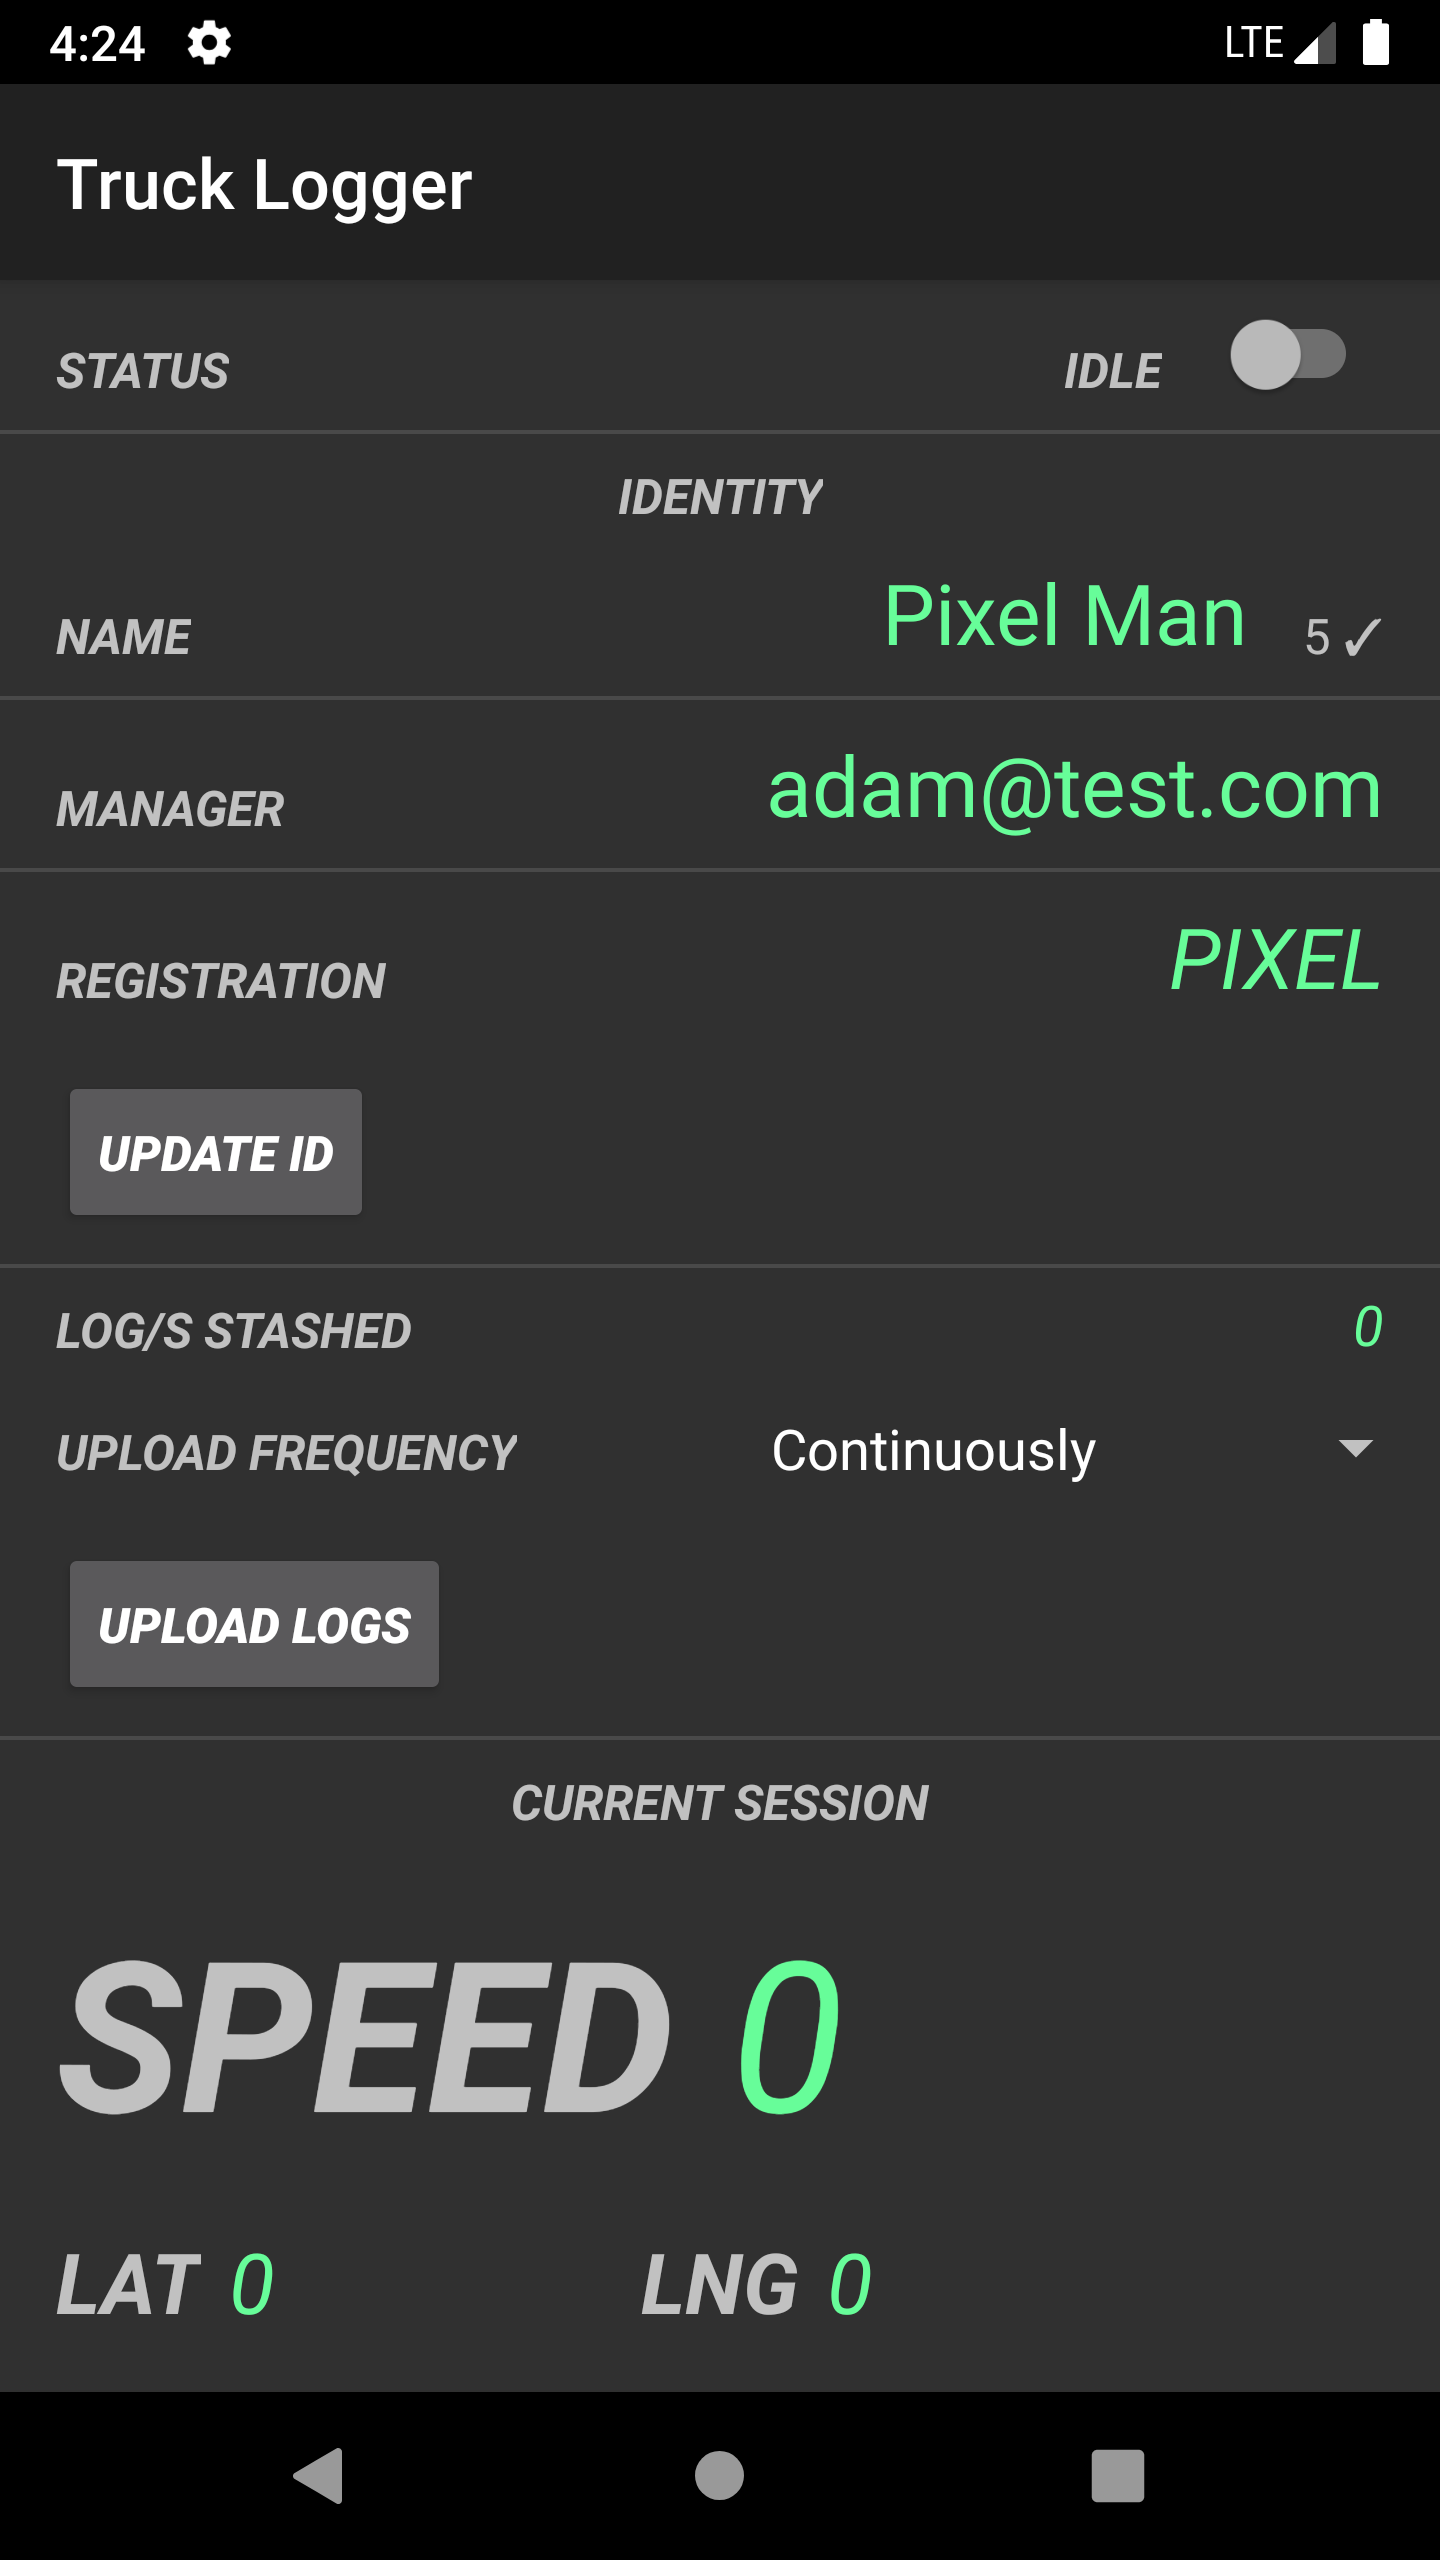
\includegraphics[height=2.5in]{android_app_idle.png}
        \label{fig:android_app_idle}
    }
    \subfigure[Running state]
    {
        \centering
        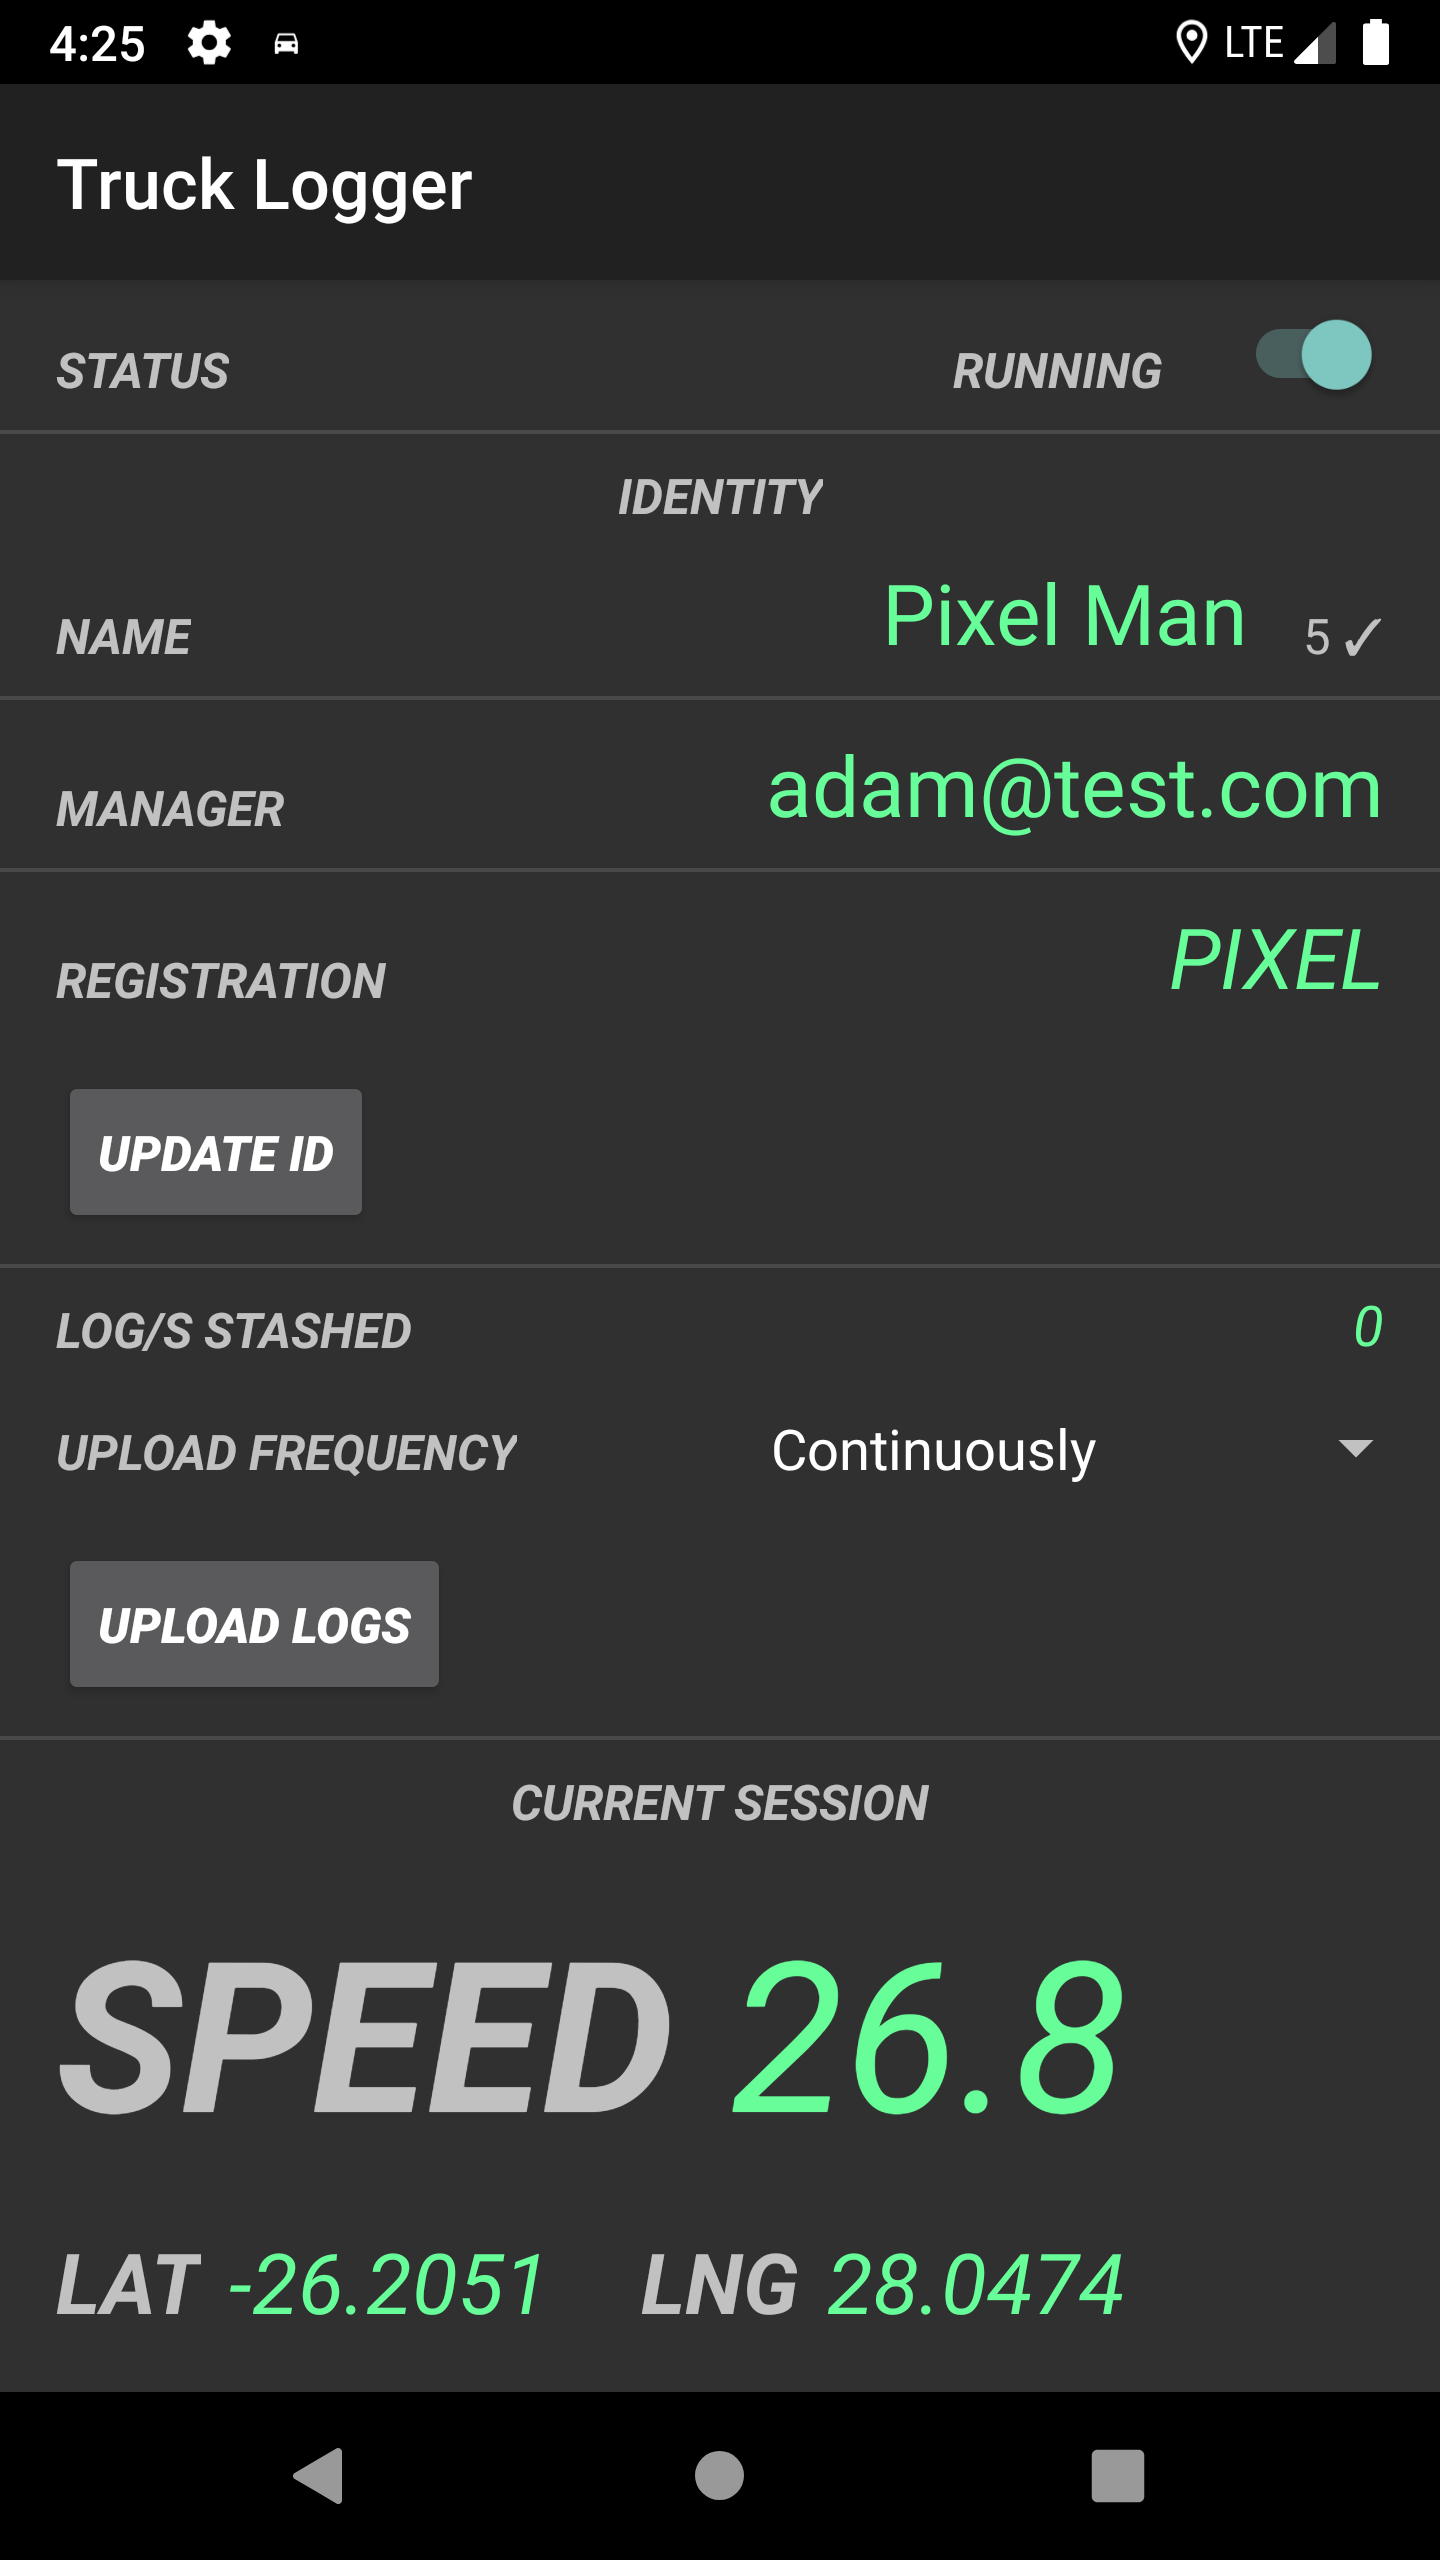
\includegraphics[height=2.5in]{android_app_running.png}
        \label{fig:android_app_running}
    }\\
    \subfigure[Background operation]
    {
        \centering
        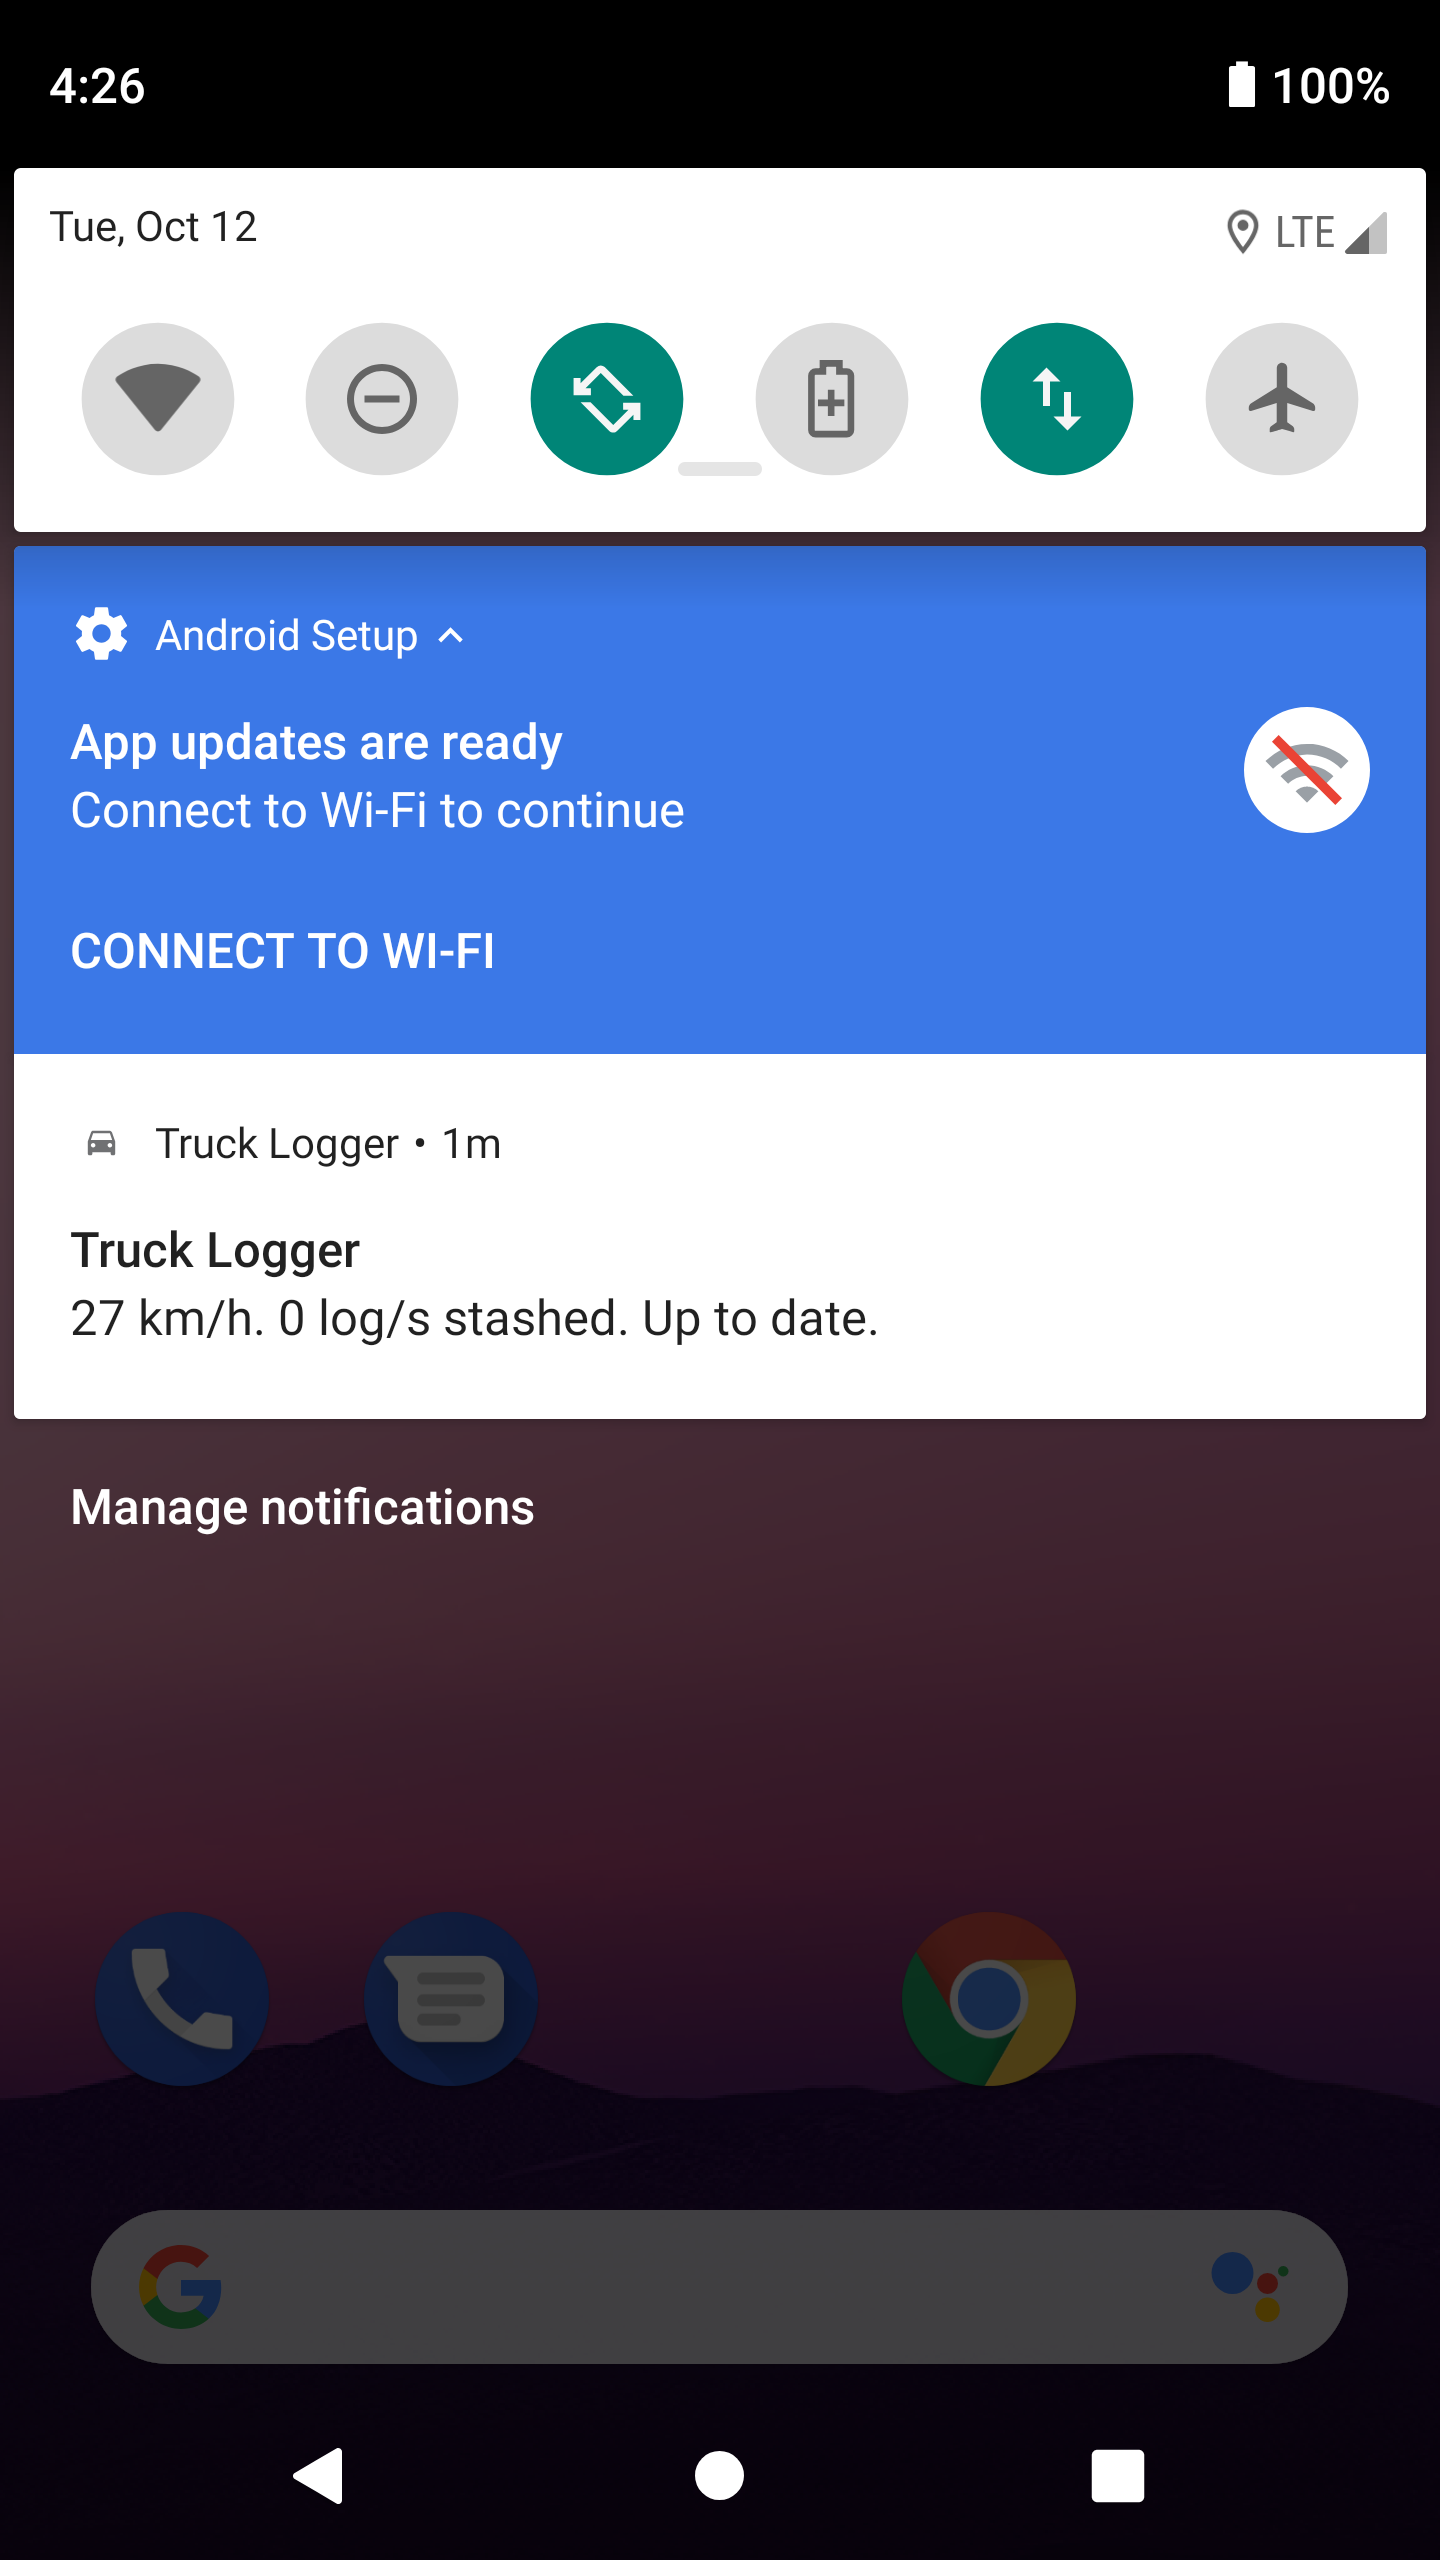
\includegraphics[height=2.5in]{android_app_background.png}
        \label{fig:android_app_background}
    }
    \subfigure[Stashing logs locally]
    {
        \centering
        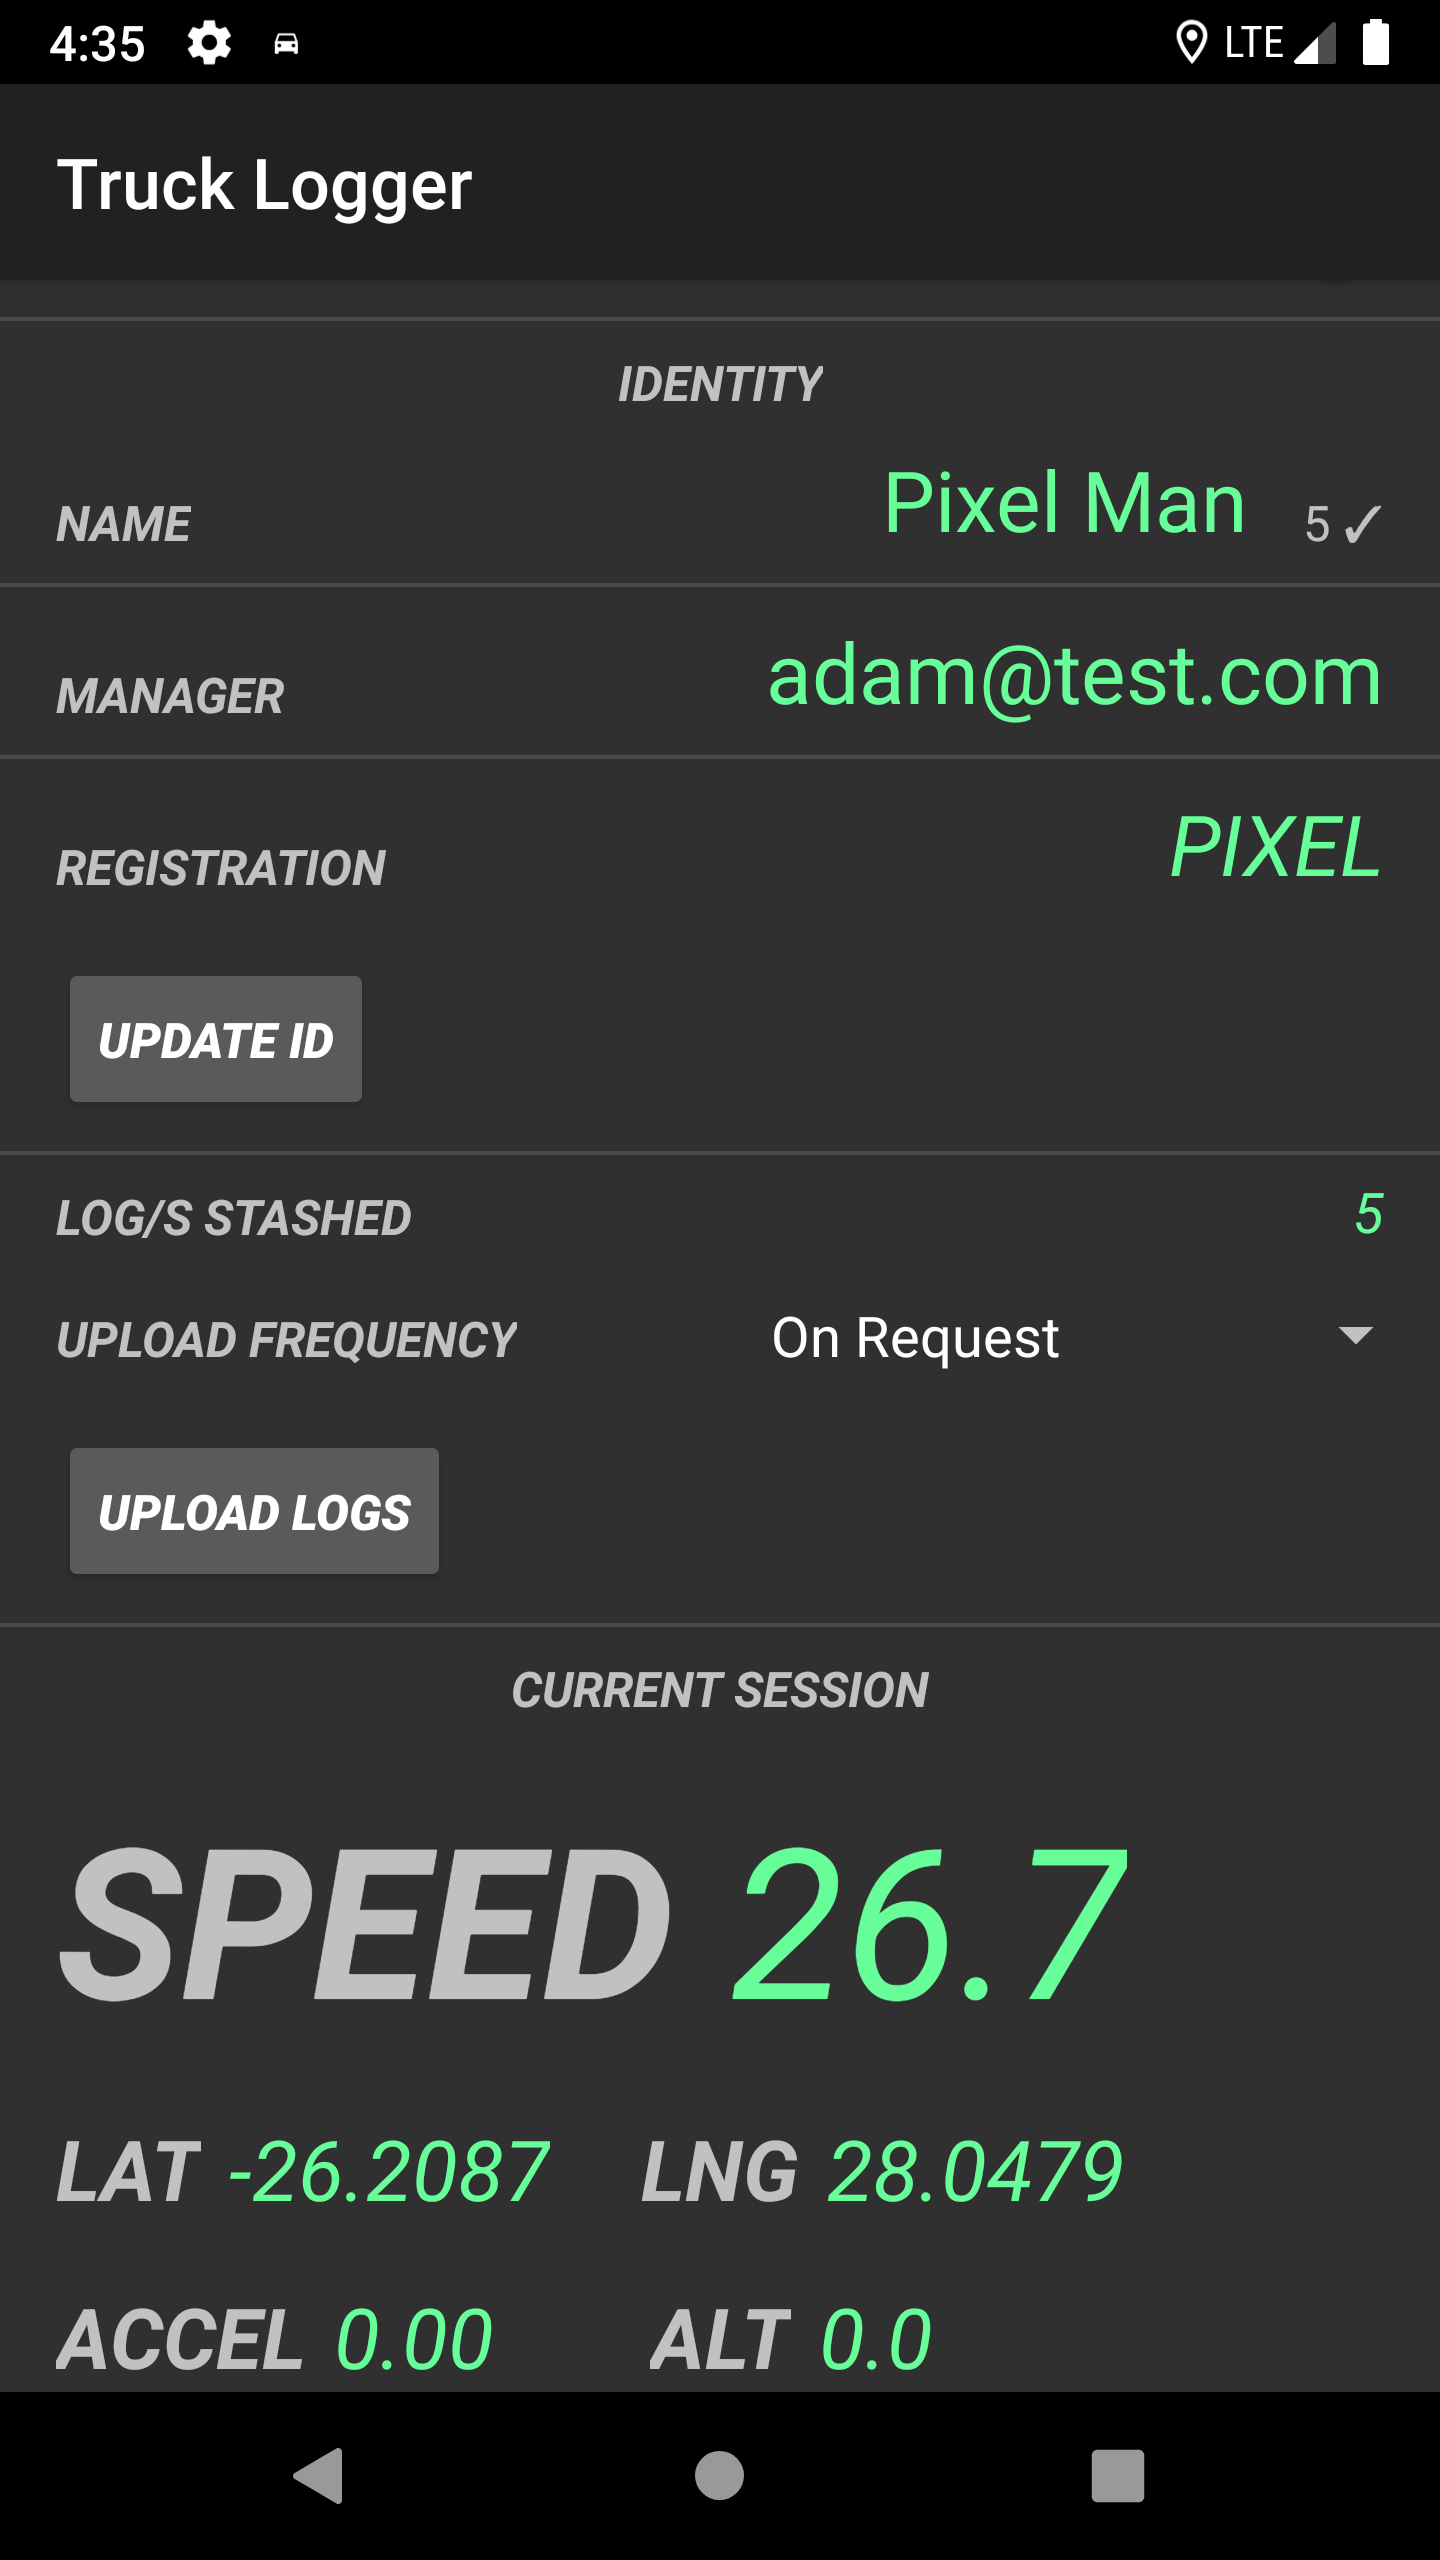
\includegraphics[height=2.5in]{android_app_stashing.png}
        \label{fig:android_app_stashing}
    }
\caption{Android application - Implemented layout}
\label{fig:android_app_implementation}
\end{figure}

The \ac{ui} provides an interface detailing \ac{id} information related to the trucker and manager.
Users can update their \ac{id} as long as they have connectivity to the server.
They can also upload all log data at any instance.

Figure \ref{fig:android_app_idle} depicts the application in an idle state.
The application performs no logging in this state.

Toggling the status check box allows the application to start logging data, as seen in figure \ref{fig:android_app_running}.
This activates the background process which polls for \ac{gps}, acceleration (provided the linear composite accelerometer if available) and altitude.
While tracking, a constant notification is displayed, indicating speed and number of logs stashed.

Depending on the upload frequency, an attempt is made to upload logs to the central server.
Otherwise logs are stashed in the SQLite database.

\subsection{\Ac{io} Server}
Low-level implementation details are included in appendix \ref{App:io_server}.
Figure \ref{fig:io_output} depicts the output of the \ac{io} server, logging request information from multiple users to standard output.

\begin{figure}[H]
\centering
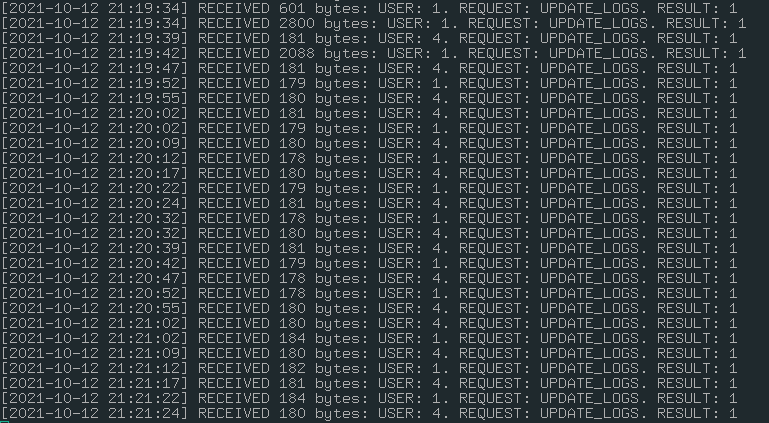
\includegraphics[scale=0.60]{io_output.png}
\caption{IO Server - Request information logged to standard output}
\label{fig:io_output}
\end{figure}

The \Ac{io} server handles \ac{ssl} connections transmitting a serialized \ac{json} payload consisting of the truckers \ac{id}, \ac{uuid} and extra data (detailed in figure \ref{fig:json_protocol}).
The \ac{uuid} is added to ensure that one trucker can be associated with a device.
Depending on the request code provided, the server processes each request appropriately.

\subsubsection{Requests}
The \ac{io} server handles various requests.
Each request type is specified by a request code, as shown in figure \ref{fig:json_protocol}.
\begin{enumerate}
\item \textbf{UPDATE ID}\\
The trucker sends a request to update their \ac{id} with a newly generated \ac{uuid}.
As long as the \textit{Verified} flag is set to false, the server will update its record of the \ac{uuid} corresponding to that trucker \ac{id}.
The manager must first set the flag to false if they need to reset the trucker's device or change the identity associated with a specific trucker.
The \textit{Verified} flag is then set to true.
All future requests must provide the \ac{uuid}.

\item \textbf{VERIFY ID}\\
This request ensures that a truckers \ac{id} and \ac{uuid} correspond in the database.
If not, the server returns a \textit{INVALID CREDENTIALS} response code.
This mechanism ensures that only one device can send logs for a corresponding trucker \ac{id}.

\item \textbf{UPDATE LOGS}\\
This request first performs logic for verifying \ac{id}s, associated with the \textit{VERIFY ID} request.
If the incoming \ac{id} is valid, the log records for the specific device are added to the database.
\end{enumerate}

\subsubsection{Responses}
The server responds with an appropriate response code, to the android requests.
\begin{enumerate}
\item \textbf{FAIL}\\
A fail code indicating the response was invalid.
\item \textbf{OK}\\
A success code indicating the response was valid.
\item \textbf{INVALID CREDENTIALS}\\
A fail code indicating that the client's \ac{id} and \ac{uuid} do not correspond.
\item \textbf{DB CONN FAILED}\\
A server error triggered by an exception when the server can't establish connection with the database.
\item \textbf{PARSE FAIL}\\
The incoming \ac{json} serialized payload was malformed and could not be deserialized.
\end{enumerate}

\subsection{Web application}
The web application is implemented using the \textit{ASP.NET Core} framework, running in Linux on the Kestrel web server.

\subsubsection{User login and signup}
Microsoft's \textit {ASP.NET Core Identity} library provides an easy automated interface for handling manager identity.
It provides user log in and sign up pages, as seen in figure \ref{fig:webapp_userhandling}.

\begin{figure}[H]
\centering
    \subfigure[Sign up]
    {
        \centering
        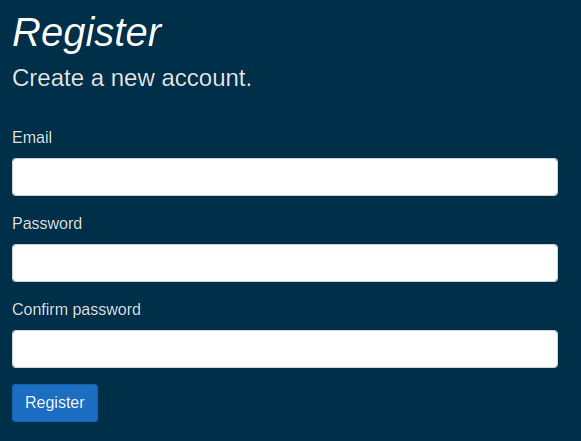
\includegraphics[width=2.5in]{webapp_signup.png}
        \label{fig:webapp_signup}
    }
    \subfigure[Log in]
    {
        \centering
        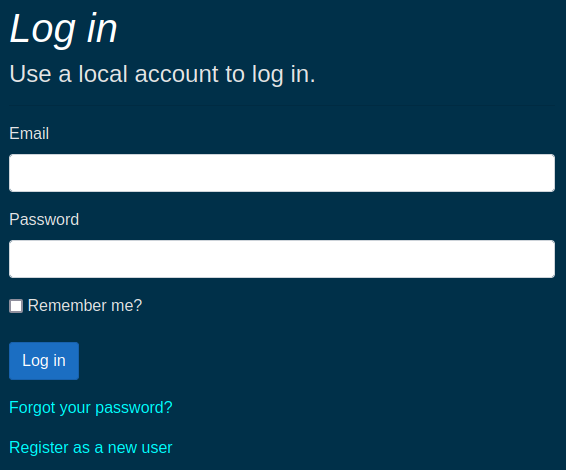
\includegraphics[height=2.5in]{webapp_login.png}
        \label{fig:webapp_login}
    }
\caption{Web application - Manager account handling}
\label{fig:webapp_userhandling}
\end{figure}

\subsubsection{Fleet viewing and management}
The Fleet Controller is implemented in handling \Ac{http} requests for serving web pages related to the manager's Fleet.
Fleet Controller methods are called when the \ac{uri} in the address bar is appended with the text \textit{Fleet}.

\begin{figure}[H]
\centering
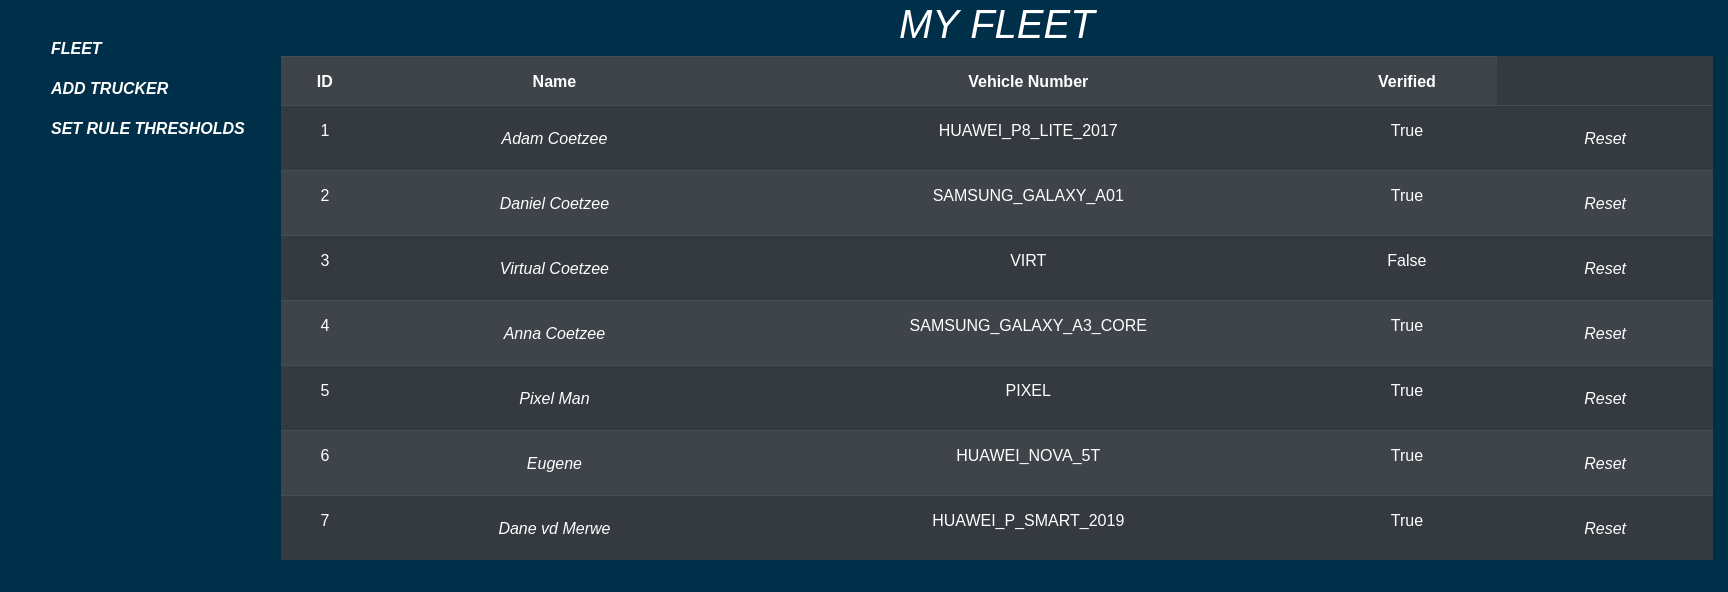
\includegraphics[width=6in]{webapp_fleet_index.png}
\caption{Web application - Fleet Index}
\label{fig:webapp_fleet_index}
\end{figure}
The Fleet Index page shown in figure \ref{fig:webapp_fleet_index} displays a list of all truckers in the manager's fleet.
The \textit{Verified} attribute indicates whether a trucker is paired to a specific device.
This attribute can be reset to allow the pairing process to be performed again for the same or a new device.

\begin{figure}[H]
\centering
    \subfigure[Add Trucker]
    {
        \centering
        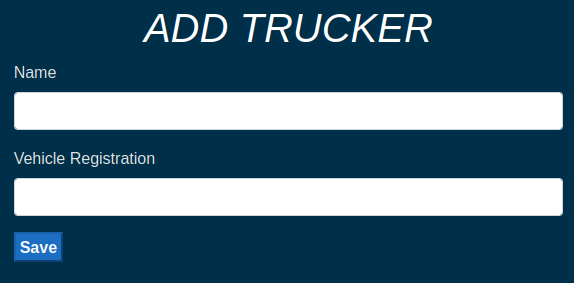
\includegraphics[width=2.5in]{webapp_add_trucker.png}
        \label{fig:webapp_add_trucker}
    }
    \subfigure[Set rules]
    {
        \centering
        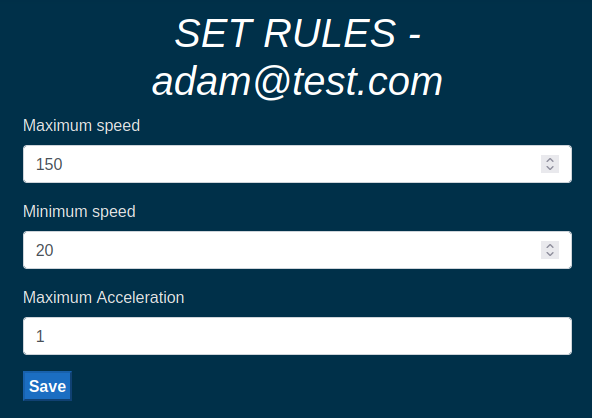
\includegraphics[height=2.5in]{webapp_set_rules.png}
        \label{fig:webapp_set_rules}
    }
\caption{Web application - Fleet management}
\label{fig:webapp_fleet_management}
\end{figure}
Figure \ref{fig:webapp_fleet_management} depicts pages implemented for adding truckers and setting rule thresholds.
They both make use of \ac{html} forms bound to the Manager and Trucker model.
\Ac{http} requests are routed to the Fleet Controller and handled by an appropriate method.

\subsubsection{Trucker activity}
\begin{figure}
\centering
    \subfigure[View Trucker]
    {
        \centering
        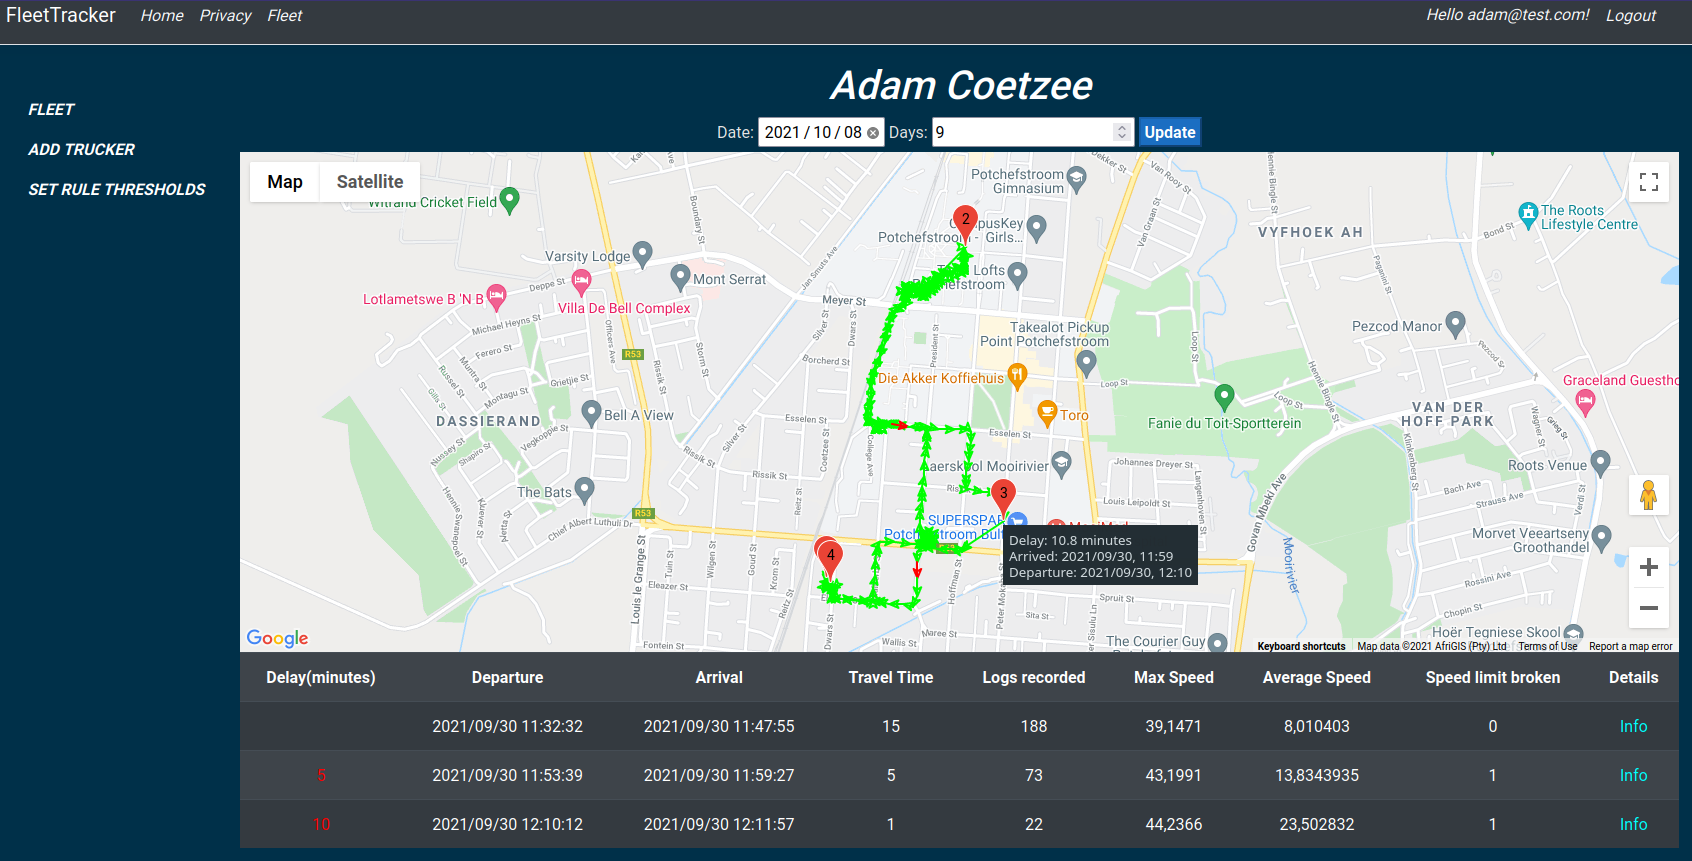
\includegraphics[width=6in]{webapp_view_trucker.png}
        \label{fig:webapp_view_trucker}
    }
    \subfigure[View Trip]
    {
        \centering
        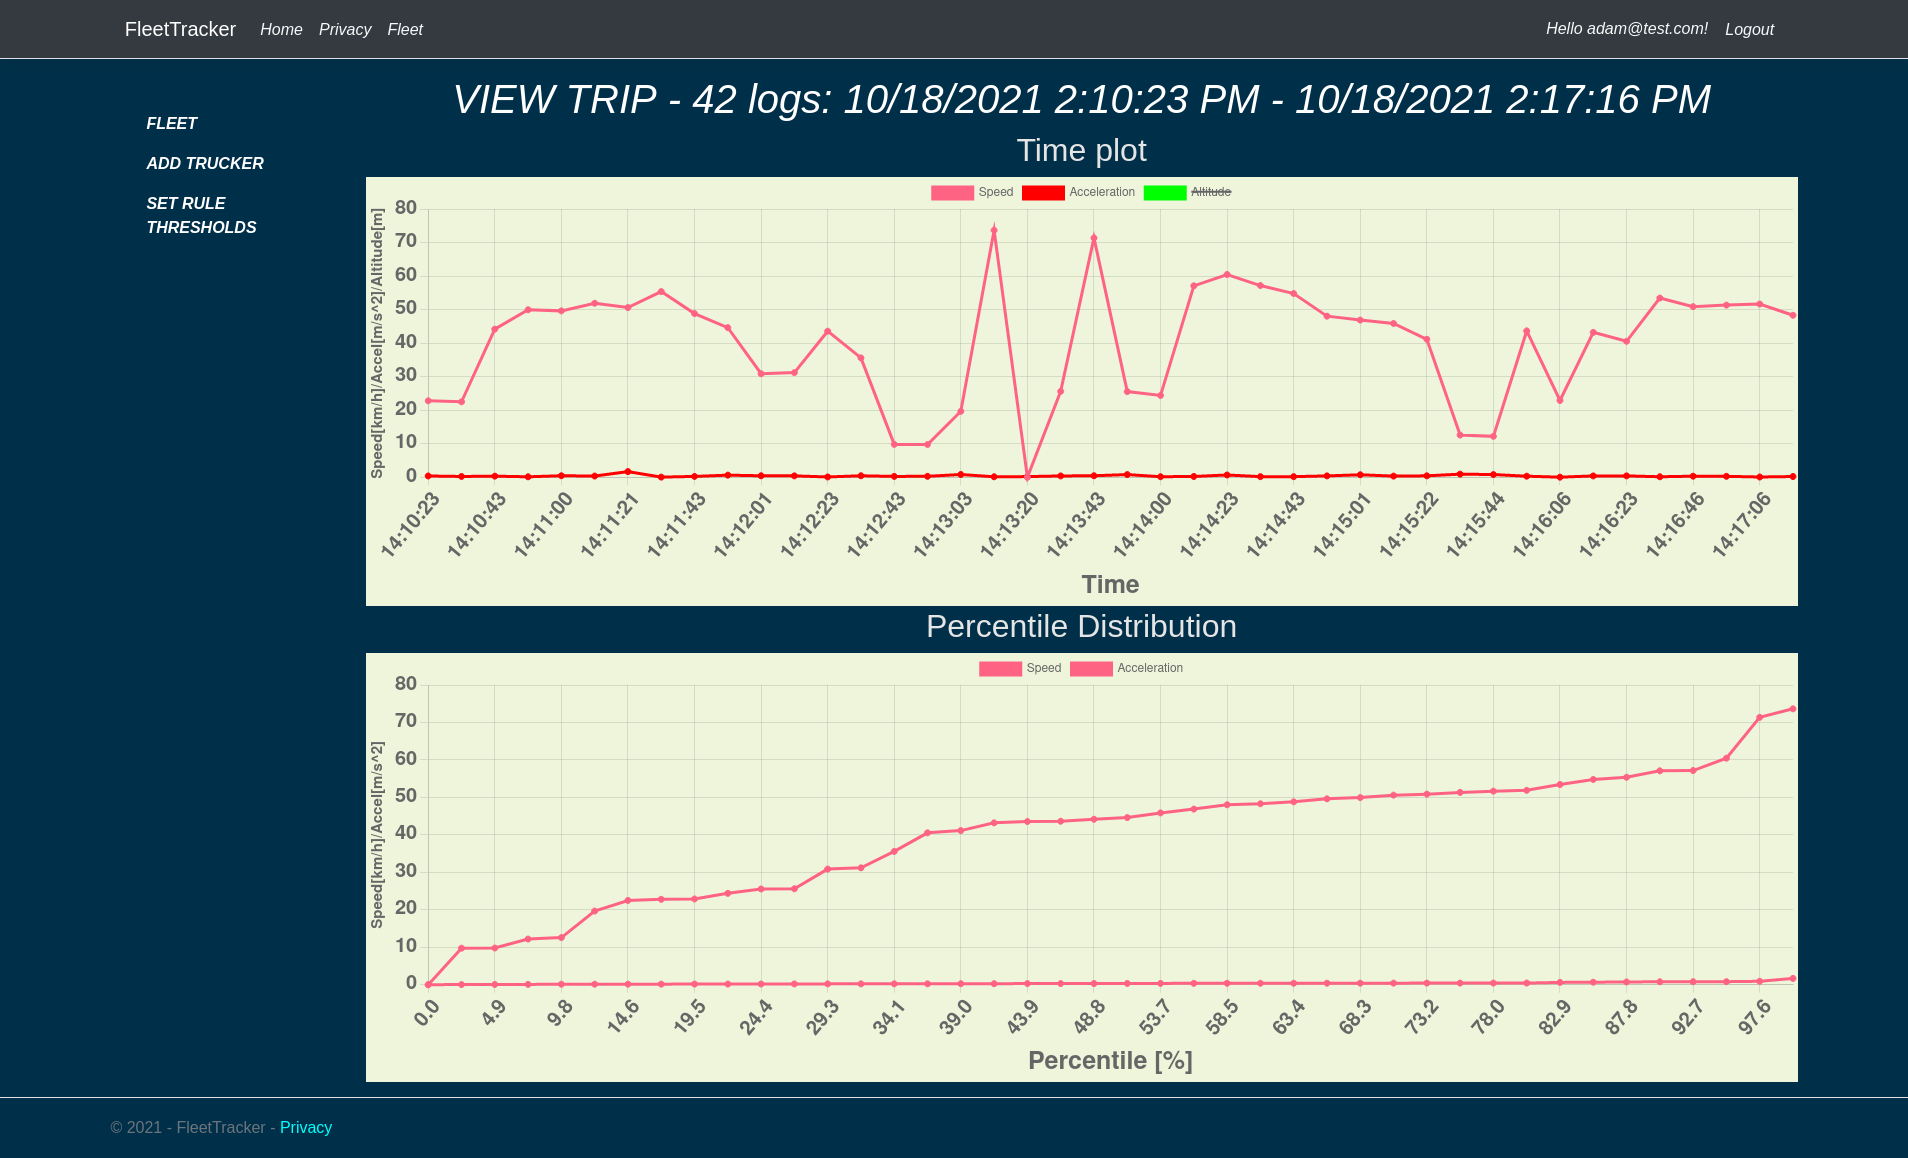
\includegraphics[width=6in]{webapp_view_trip.png}
        \label{fig:webapp_view_trip}
    }
\caption{Web application - Trip collection and information}
\label{fig:webapp_trucker_details}
\end{figure}
Figure \ref{fig:webapp_trucker_details} (next page) details the interface for viewing trucker activity.

Figure \ref{fig:webapp_view_trucker} provides a time adjustable page which groups the logs into individual trips.
A map is rendered (using the Google JavaScript \Ac{api}) with routes physically drawn in the map, using arrows.
If the defined speed limit is broken, the arrows are drawn in red.
Stopping points are indicated with markers labeled in chronological order.
Hovering over a stop label indicates how long the trucker had stopped at a given location.
A table is rendered displaying this information.

Figure \ref{fig:webapp_view_trip} allows a more detailed view of an individual trip between two markers.
Time plots indicate give speed, acceleration and altitude plots which vary with time as truckers carry out their trips.
A percentile plot is included to visualize the spread of speed and acceleration.
This allows managers to visualize what portions of the trip was driven with specific behavior.

\pagebreak
\subsection{Deployment}
The web application and \ac{io} server are deployed to a Linux \ac{vps} with access to a static \ac{ip} address and domain name.
A non-profit \ac{ca} Lets Encrypt provides \ac{ssl} certificates, which are required for Android applications which make use \ac{ssl} communication.

Docker containers are created and used for used for deploying the MySQL database and \ac{io} server. 
They are useful for managing dependencies and preventing unwanted changes to the host server.

A link is provided for downloading the Android application as an \ac{apk} file.

\pagebreak
